\section{Decision Model and Evaluation Criteria}
\label{sec:model}

Figure~\ref{fig:overview} separates the information available when the forecast is issued, when reserve is requested, and when the outcome is observed. Selected telemetry joins the fixed forecast and common inputs at decision time. The fitted estimator and historical correction then produce a reserve request; future power is used only to assess that request.

\begin{figure*}[!t]
\centering
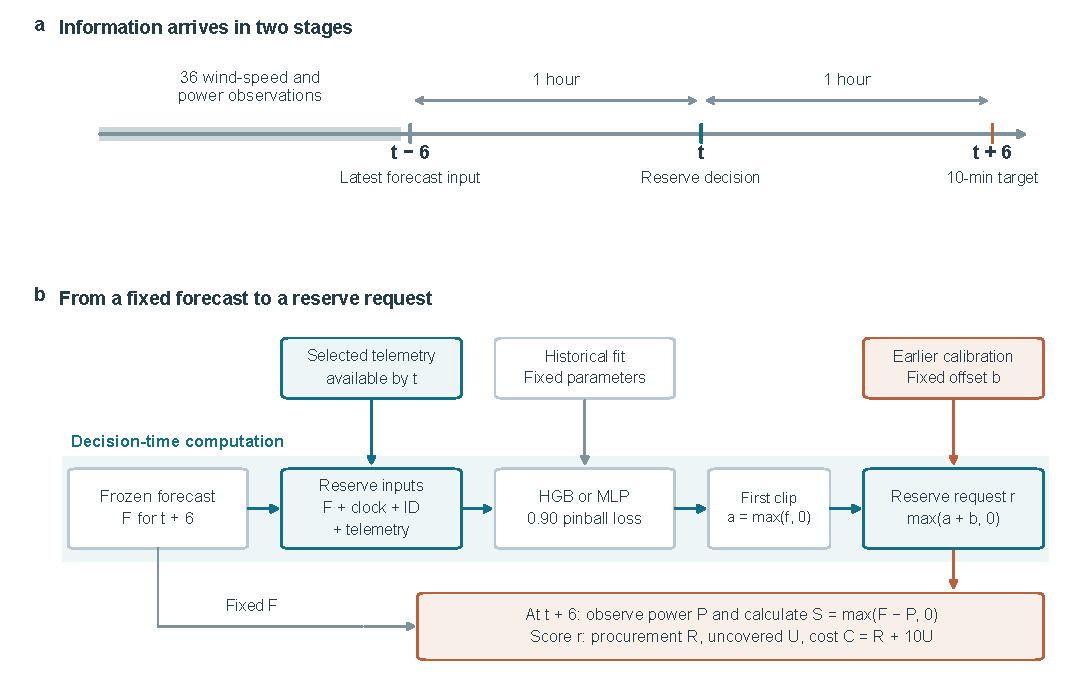
\includegraphics[width=\textwidth]{figures/v14/fig1_architecture.pdf}
\caption{Overall architecture and information timing. (a) On a ten-minute grid, the forecast uses 36 wind-speed and active-power observations ending at $t-6$. Reserve is requested at $t$ for the ten-minute target at $t+6$. The latest forecast input and the target are two hours apart; the reserve lead is one hour. The older history segment is schematic. (b) Available telemetry augments the forecast, clock and turbine identifier. The estimator output is clipped at zero, the signed historical offset is added, and the result is clipped again. Parameters and offsets remain fixed during evaluation. Future power enters shortfall and cost accounting only. This is a controlled information arrangement, not a measured communication delay.}
\label{fig:overview}
\end{figure*}

\subsection{Forecast commitment and shortfall loss}
Let $t$ denote the reserve decision time on a ten-minute grid, and let $i$ identify a turbine. The common forecast $F_{i,t}$ uses 36 wind-speed and active-power observations ending at $t-6$ to predict power at $t+6$. Thus, the reserve decision precedes the target by one hour, while the forecast target lies two hours after its latest input. The forecast remains fixed when the reserve inputs change. This controlled information arrangement separates the upstream forecast from the additional telemetry supplied at decision time. The target is one ten-minute interval. For its measured active power $P_{i,t+6}$, forecast shortfall is
\begin{equation}
 S_{i,t}=\max(F_{i,t}-P_{i,t+6},0).
\label{eq:shortfall}
\end{equation}

A reserve policy $m$ requests nonnegative reserve $r^m_{i,t}$ in kW. With a ten-minute interval $\Delta=1/6$ h, procured energy and uncovered shortfall are $R^m_{i,t}=\Delta r^m_{i,t}$ and $U^m_{i,t}=\Delta\max(S_{i,t}-r^m_{i,t},0)$. We evaluate their asymmetric decision loss and the associated event indicator as
\begin{equation}
 \begin{aligned}
 C^m_{i,t}&=R^m_{i,t}+\rho U^m_{i,t},\quad \rho=10,\\
 V^m_{i,t}&=\mathbf{1}\{S_{i,t}>r^m_{i,t}\}.
 \end{aligned}
\label{eq:loss}
\end{equation}

The penalty ratio makes an uncovered deficit more costly than procuring the same energy as reserve. Cost is expressed as a kWh-equivalent proxy per valid turbine interval; procurement and uncovered shortfall are expressed in kWh. For the corresponding unconstrained newsvendor decision, the expected loss is minimized at the conditional $(1-1/\rho)=0.90$ shortfall quantile. This relation motivates quantile regression for the reserve request \cite{koenker1978regression,soares2016}.

\subsection{Reserve estimators and historical offsets}
Each learned policy receives four common inputs: the point forecast, sine and cosine of time of day, and normalized turbine identifier. Telemetry configurations add measurements to these shared inputs. We use histogram gradient boosting (HGB) and a multilayer perceptron (MLP), both trained with the 0.90 pinball loss. HGB uses 100 boosting iterations and at most 15 terminal leaves. The MLP has two rectified linear hidden layers containing 64 and 32 units. Preprocessing is fitted on training data; complete settings are given in Supplementary Section S3.

Let $a^m_{i,t}=\max(f_m(x_{i,t}),0)$ denote the nonnegative raw reserve estimate for input vector $x_{i,t}$. A signed offset is calculated from historical shortfall residuals at calibration level $q$:
\begin{equation}
 \begin{aligned}
 b_{m,q}&=\operatorname{Quantile}^{\mathrm{higher}}_q
 \{S_{i,t}-a^m_{i,t}:(i,t)\in\mathcal D_{\rm cal}\},\\
 r^{m,q}_{i,t}&=\max(a^m_{i,t}+b_{m,q},0).
 \end{aligned}
\label{eq:offset}
\end{equation}

The $q$ value indexes residual-offset calibration, rather than a separately trained quantile model. The calibration grid contains $q=0.90,0.925,0.95,0.975,0.99$. The primary Hill of Towie comparison uses $q=0.95$; the secondary finite-family analysis uses $q=0.925$. Five fitted instances use seeds 201--205, with matched training samples across input configurations.

Figure~\ref{fig:decisionexample} illustrates this construction using a complete recorded day. The request follows the nonnegative estimator output with the same historical offset at every decision. Subsequent shortfalls reveal both covered and uncovered outcomes, while the offset grid shows the calibration choices made before evaluation.

\begin{figure*}[!t]
\centering
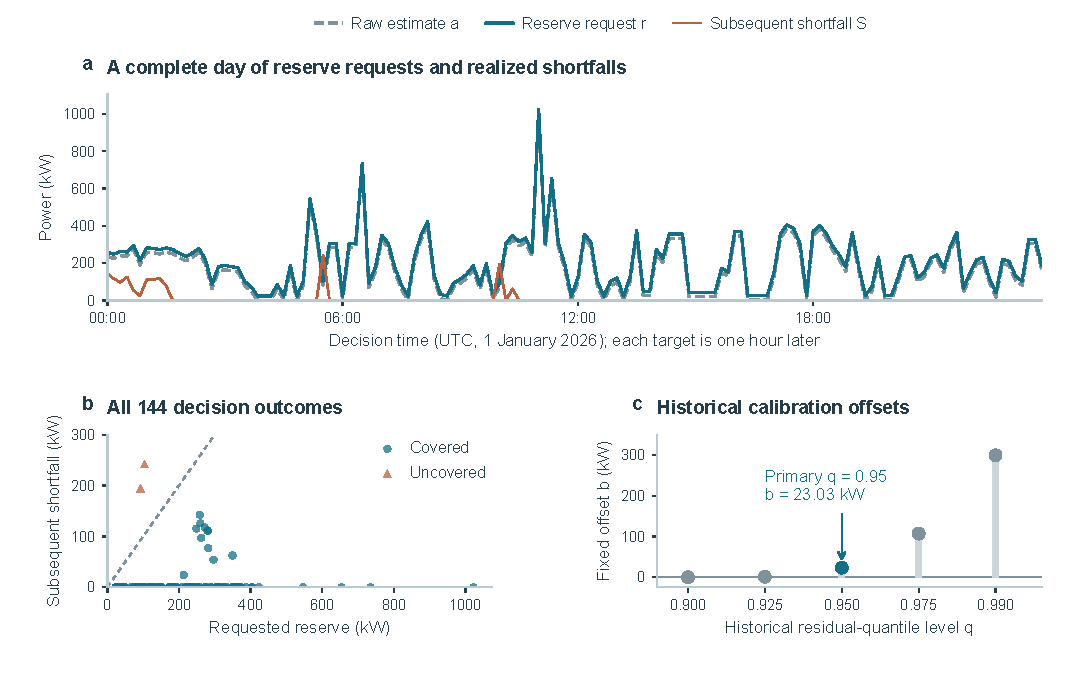
\includegraphics[width=\textwidth]{figures/v14/fig2_decision_example.pdf}
\caption{Reserve construction in a recorded day at Hill of Towie: turbine 1, 1 January 2026, P1/HGB, seed 201, $q=0.95$. (a) All 144 raw nonnegative estimates, final requests and subsequent shortfalls are retained. Shading marks shortfall above the request. The horizontal axis is decision time; each outcome belongs to the target one hour later. (b) Every request is paired with its realized shortfall. The dashed equality line separates covered circles from uncovered triangles; the two axes have different ranges to show the observed outcomes clearly. (c) The five stored historical residual offsets, with the primary $q=0.95$ offset highlighted. These are calibration choices, not confidence intervals or separately fitted quantile models.}
\label{fig:decisionexample}
\end{figure*}

\subsection{Fixed-reference requirements and resource order}
For candidate $m$ and fixed reference $b$, define relative mean-cost difference $D_C=\bar C_m/\bar C_b-1$. A rule is qualified if
\begin{equation}
 \begin{aligned}
 \operatorname{UCB}_{.95}(D_C)&\le 0.02,\\
 \max_s\operatorname{UCB}_{.95}(V_{m,s})&\le0.10,\\
 \max_s\operatorname{UCB}_{.95}(V_{b,s})&\le0.10.
 \end{aligned}
\label{eq:criteria}
\end{equation}

Here $s$ indexes the five fixed fits, and UCB denotes the upper bound from the simultaneous procedure below. The 2\% cost margin defines the accepted premium for input reduction. The event-rate cap applies to every fit of both candidate and reference. These declared comparison criteria assess cost and event frequency; procurement and uncovered-shortfall magnitude provide the accompanying action accounting.

Historical selection uses risk bounds and mean cost to choose the offset for each fitted recipe. Resource-minimal recipes are retained from the historically identified near-optimal set. The richer reference is selected from risk-qualified three-channel recipes on the same historical period. Both choices are then held fixed during subsequent evaluation.

For finite-family assessment, policies are ordered lexicographically by added telemetry channels, learned predictor passes and raw input width. Passing the fixed-reference criteria establishes sufficiency relative to that reference. A resource minimum within the registered finite family additionally requires exclusion of every strictly smaller candidate.

\subsection{Paired block inference}
We estimate uncertainty using 20,000 circular resamples of contiguous UTC weather days \cite{kunsch1989jackknife}. The primary block length is three days, with one-day and seven-day sensitivity analyses. The same day blocks are used for all paired policies and fits. Daily numerators and valid-record denominators are resampled together, then pooled to calculate interval-level means. A maximum standardized deviation gives an approximate simultaneous 95\% envelope for each declared comparison family. Studies and evaluation windows have separate families. Weather days are the sampling units, and the five fitted instances remain fixed. Supplementary Section S4 specifies the families and random seeds.
